\section*{Exercice 129 -- PFD -- Robot chirurgical}
\setcounter{exo}{0}
%CCS PSI 2015

\begin{obj}
Déterminer les équations du mouvement du bras esclave sous la 
$A\vect{\ddot{q}}+B\vect{\dot{q}}+C\vect{q}=\vect{F}$.
\end{obj}


Trois mouvements de l’outil existent :
\begin{itemize}
\item la rotation du corps de l’outil 7’ par rapport à 6’, autour de $\axe{T}{y_2'}$, ce mouvement ne sera pas étudié ici ;
\item la rotation du corps d’outil 7’ par rapport au bâti 0 autour de $\axe{T}{z_0}$. La transmission de ce mouvement de
l’actionneur dédié jusqu’à 7’ est assurée par la structure globale étudiée aux questions précédentes, associée
à une came circulaire liée au bâti sur laquelle roule sans glisser le galet 9’ ;
\item la translation du corps d’outil 7’ par rapport au porte-outil 6’. La transmission de ce mouvement de l’actionneur
dédié jusqu’à 7’ est assurée par un système complexe de câbles donné dans la figure suivante.
\end{itemize}


\begin{center}
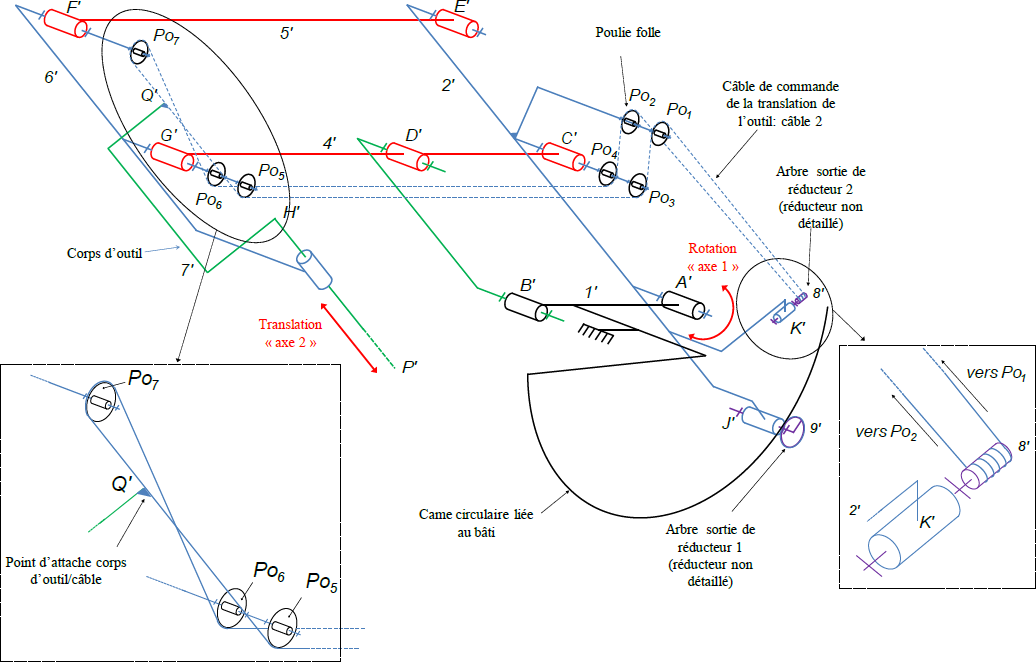
\includegraphics[width=\linewidth]{992_02}
\end{center}

Les trois degrés de liberté du corps d’outil sont obtenus au moyen de la structure retenue (figures précédente et suivante) à
laquelle deux axes asservis sont associés. Avec cette structure, une variation de l’angle $\delta(t)$ n’entraîne pas une
variation de $\lambda(t)$. Les deux axes sont donc indépendants géométriquement.


\begin{center}
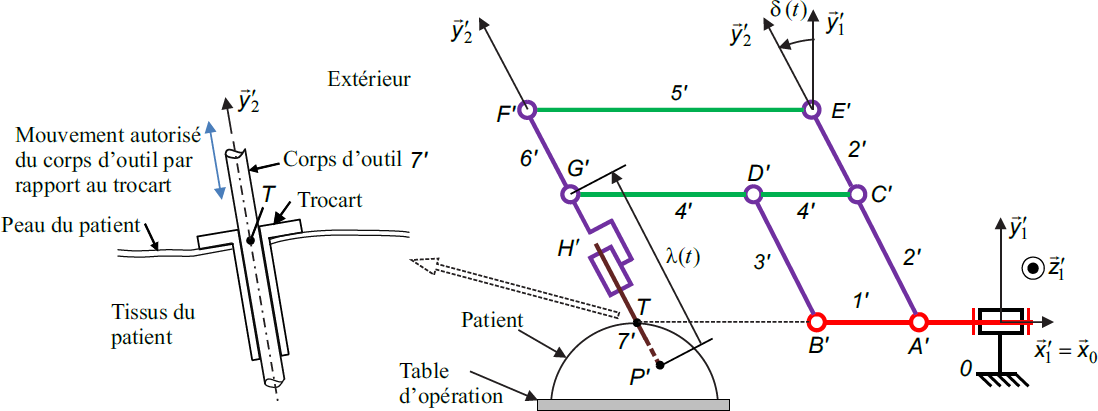
\includegraphics[width=\linewidth]{992_03}
\end{center}

Les équations du mouvement des axes 1 et 2 sont nécessaires pour réaliser une synthèse
des correcteurs. Dans le cadre de ce sujet, on se limite à la détermination de l’équation du mouvement de l’axe
2 (décrivant l’évolution de la grandeur $\lambda(t)$).

La figure suivante montre le détail du moto-réducteur 2. Pour simplifier, on considère que le câble est enroulé sur un
demi-tour du tambour 8’. $\theta_2$ est l’angle du rotor du moteur par rapport à son stator 2’.


\begin{center}
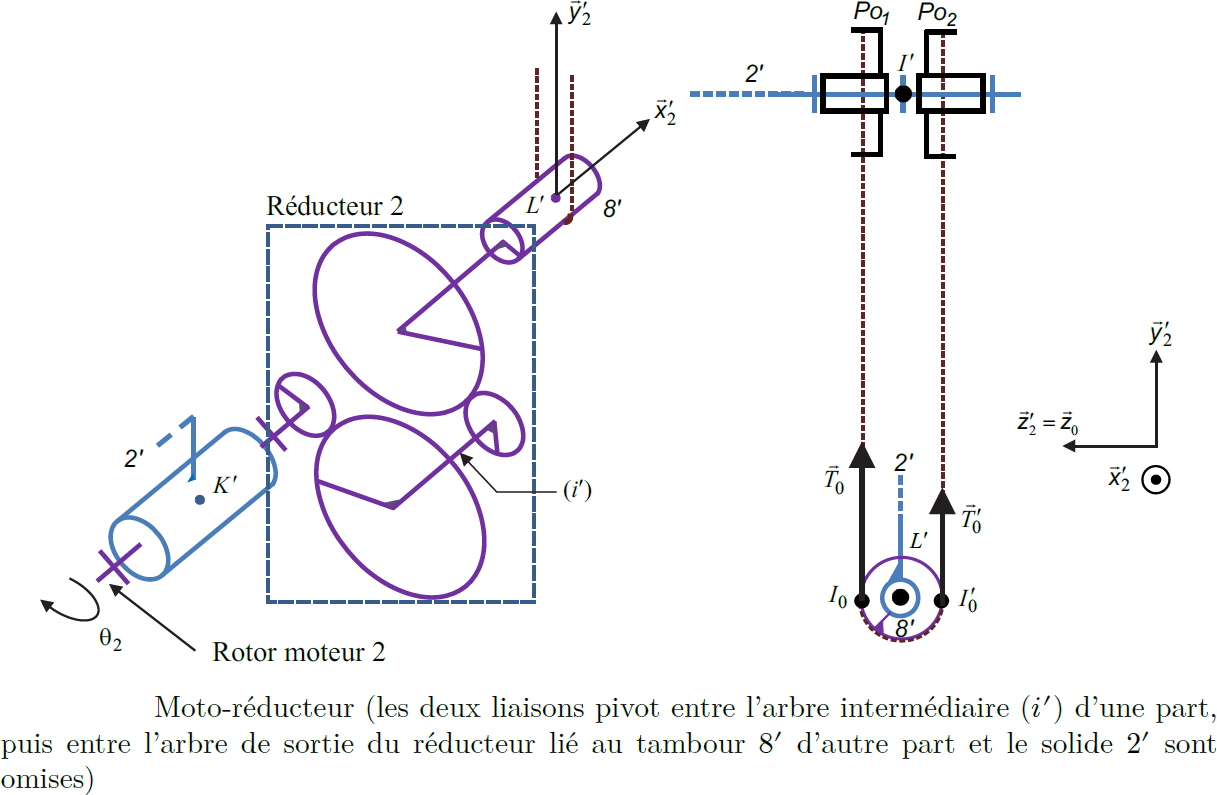
\includegraphics[width=\linewidth]{992_01}
\end{center}

\begin{itemize}
\item Le repère $\rep{0}$ est supposé galiléen. La verticale ascendante est $\vect{y_0}$.
%\item Le torseur des actions mécaniques transmissibles par une liaison d’un solide $i$ sur un solide $j$, réduit en un
%point $M$, est noté : $\torseurstat{T}{i}{j}=\torseurl{\vectf{i}{j}}{\vectm{M}{i}{j}}{M} = \torseurcol{X_{ij}}{Y_{ij}}{Z_{ij}}{L_{ij}}{M_{ij}}{N_{ij}}{M,\rep{0}}$.
%\item Le torseur dynamique d’un solide $i$ par rapport au repère $\rep{0}$, réduit en un point $M$, est noté : 
% $\torseurdyn{i}{j}=\torseurl{\vectrd{i}{j}}{\vectmd{M}{i}{j}}{M}$
\item La force exercée par le tissu humain sur le corps d’outil 7’ est modélisée par le glisseur $\axe{P'}{F_e}$
avec $\vect{F_e}=F_x(t)\vect{x_2'}+F_y(t)\vect{y_2'}$.
\item L’effort du corps d’outil 7’ sur le câble est modélisé par le glisseur $\axe{Q'}{F}$, $Q'$ étant le point
d’attache entre le corps d’outil 7’ et le câble avec $\vect{F}=F(t)\vect{y_2'}$.
\item L’action de la pesanteur sur 7’ est négligée devant les efforts mis en jeu.
\item $H'$ est le centre d’inertie de 7’, $m'_7$ sa masse et $\vect{P'H'}=l_0\vect{y_2'}$.
\item L’action du moteur 2 (utilisé pour le mouvement de translation de l’outil correspondant à l’« axe 2 ») est
modélisée par un couple pur : $\vect{C_{m2}}=C_{m2}(t)\vect{x_2'}$.
\item On note  $\vect{C_{\text{red}}}=C_{\text{red}}\vect{x_2'}$, le couple moteur ramené à l’arbre de sortie du réducteur 2 solidaire de 8’. Une étude préalable a permis d’obtenir la relation
$C_{\text{red}}=\dfrac{C_{m2}}{k_2}$ ($k_2$ étant le rapport de transmission du réducteur).
\item Les actions mécaniques du câble sur 8’ sont modélisées par deux glisseurs en $I_0$ et $I_0'$ : 
$\axe{I_0}{T_0}$  et $\axe{I_0'}{T_0'}$ avec
$\vect{T_0}=\left( T_t + \dfrac{F(t)}{2}\right)\vect{y_2'}$
et $\vect{T'_0}=\left( T_t - \dfrac{F(t)}{2}\right)\vect{y_2'}$ où
$T_t$ représente la valeur algébrique de la pré-tension dans les câbles pour assurer qu’ils soient tendus constamment en cours d’opération, quelle que soit la valeur de $F(t)$.
\item Le rendement du réducteur est supposé unitaire. Le moment d’inertie du rotor du moteur 2 et des pièces du réducteur 2 sont négligées. La masse des câbles est négligée.
\end{itemize}
On se propose en premier lieu de déterminer l’expression du couple moteur $C_{m2}(t)$ en fonction de  $F_y(t)$ et des paramètres du problème tel que
$$C_{m2}(t)=v_1\left( 
F_y(t)+m_7'\left( \dfrac{\dd^2 \lambda(t) }{\dd t^2}+v_2 \left( \dfrac{\dd \delta(t) }{\dd t}\right)
\right)\right)
$$
où $v_1$ et $v_2$ sont des termes à expliciter en fonction de
$k_2$, $r_8'$, $l_0$, $h_2$ et $\lambda$.
Le tableau du document réponse donne en partie la démarche de résolution.


\subparagraph{}
\textit{Compléter le tableau du document réponse et justifier, sur la copie, le choix du théorème utilisé (équation scalaire) associé à chaque isolement, sans faire aucun calcul.}
\ifprof
\begin{corrige}
\end{corrige}
\else
\fi


\subparagraph{}
\textit{Mettre en \oe{}uvre la démarche proposée pour chaque isolement en détaillant les calculs et exprimer littéralement $v_1$ et $v_2$ de l’expression de $C_{m2}(t)$ donnée plus haut.}
\ifprof
\begin{corrige}
\end{corrige}
\else
\fi

